\ffigbox[\FBwidth]{%
\caption{\centering Complémentaire du graphe \(P_4\)}\label{Fig:exam_blanc_ex_5_1_a}
}{
    \fbox{
        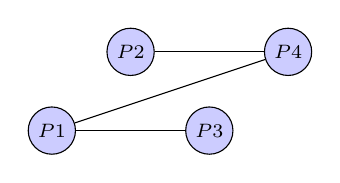
\begin{tikzpicture}[scale=1, main node/.style={circle, draw, fill=blue!20, inner sep=1pt, font=\scriptsize, minimum size=6mm}]
            % les sommets initiaux
            \node[main node] (P1) at (0,0) {\(P1\)};
            \node[main node] (P2) at (1,1) {\(P2\)};
            \node[main node] (P3) at (2,0) {\(P3\)};
            \node[main node] (P4) at (3,1) {\(P4\)};

            % les aretes
            \draw[] (P1) -- (P3);
            \draw[] (P1) -- (P4);

            \draw[] (P2) -- (P4);
        \end{tikzpicture}
    }
}
